\documentclass[11pt]{article}

\usepackage{sbc-template}
\usepackage{graphicx,url}
\usepackage[utf8]{inputenc}
\usepackage[brazil]{babel}
%\usepackage[latin1]{inputenc}  

     
\sloppy

\title{Simulação Estocástica de Epidemias Globais em Grafos Multiescala: Modelagem, Algoritmos e Validação Empírica}

\author{João Prado Campos\inst{1}, Fillipe Gabriel Costa Araujo\inst{1}, Daniel Bony Costa Garcia\inst{1},\\
Henrique Pereira Resende Rocha\inst{1}, Luiz Felipe Ribeiro Souza\inst{1}}

\address{Instituto de Ciências Exatas e Informática\\
  Pontifícia Universidade Católica de Minas Gerais (PUC Minas)\\
  Belo Horizonte -- MG -- Brasil
}

\begin{document} 

\maketitle

\begin{abstract}
  This paper presents a network epidemic simulator, developed for a Graph Theory course, that represents the world population as a single graph. Each country is a set of vertices proportional to its population, connected by geometric proximity, and countries are linked via OpenFlights flight routes. Propagation follows a stochastic compartmental model (S, E, I, R, and D) with automated isolation and vaccination, and the same graph reproduces real pandemics using public data. The graph structure and algorithms were implemented by the group, complete with complexity analysis, and a desktop application displays the progression on a map.
\end{abstract}
     
\begin{resumo} 
  Este artigo apresenta um simulador de epidemias em redes, desenvolvido na disciplina de Teoria dos Grafos, que representa a população mundial por um grafo único. Cada país é um conjunto de vértices proporcional à sua população, ligados por proximidade geométrica, e os países se conectam pelas rotas aéreas do OpenFlights. A propagação segue um modelo compartimental estocástico (S, E, I, R e D) com isolamento e vacinação automáticos, e o mesmo grafo reproduz pandemias reais a partir de dados públicos. A estrutura de grafo e os algoritmos foram implementados pelo grupo, com análise de complexidade, e uma aplicação desktop exibe a evolução no mapa.
\end{resumo}


\section{Introdução e Contextualização}

Entender como uma doença se espalha depende tanto do comportamento do agente infeccioso quanto da estrutura de contatos entre as pessoas. Os modelos compartimentais clássicos, derivados do trabalho de Kermack e McKendrick~\cite{kermack1927}, descrevem a epidemia por equações diferenciais sobre o model SIR (Suscetíveis, Infectados e Recuperados) e assumem mistura homogênea, isto é, que todo indivíduo tem a mesma chance de ser infectado. Essa hipótese, apesar de ser a base para os estudos matemáticos epidemológicos modernos, deixa de fora justamente o que mais diferencia uma epidemia de outra: redes reais têm hubs, aglomerações e poucas conexões entre comunidades, e a topologia altera de forma marcante o limiar epidêmico e o ritmo de propagação~\cite{pastor2015}.

Em escala global, a malha de transporte aéreo é o principal canal de disseminação entre países. Brockmann e Helbing~\cite{brockmann2013} mostram que a chegada de uma epidemia a um país é descrita melhor pela distância efetiva na rede de voos do que pela distância geográfica, o que justifica tratar o problema como um problema de grafos: caminhos mínimos, componentes conexos, pontes e comunidades têm interpretação epidemiológica direta. Medidas como isolamento e vacinação também têm efeitos que variam conforme quem é isolado ou vacinado e conforme o lugar que as populações ocupam na rede.

\subsection{Problema e objetivos}

Este trabalho apresenta o desenvolvimento de uma ferramenta computacional para simular e explorar a propagação de doenças em redes. O sistema representa a população mundial por um grafo único e permite ajustar parâmetros como contágio, recuperação, mortalidade e isolamento. Os objetivos são:

\begin{itemize}
  \item simular a propagação de uma epidemia sobre o grafo, com parâmetros definidos pelo usuário antes do início da execução;
  \item reproduzir visualmente pandemias reais (COVID-19, Ebola, H1N1 e SARS) a partir de datasets públicos, sobre o mesmo grafo global;
  \item aplicar e analisar, no contexto da epidemia, algoritmos de grafos implementados pelo grupo (busca em largura e em profundidade, componentes conexos, Dijkstra, pontes e articulações de Tarjan, agrupamento, centralidade e comunidades), com análise de complexidade;
  \item oferecer uma aplicação desktop com visual inspirado no jogo \emph{Plague Inc.}, em que o mapa muda de cor conforme o contágio. A inspiração é apenas visual, não de comportamento.
\end{itemize}

A ferramenta é demonstrativa: o usuário configura o cenário antes de iniciar e depois apenas assiste, sem alterar o rumo da epidemia. Por isso é um simulador didático, sem pretensão de previsão epidemiológica nem de apoio a decisões de saúde pública.

\subsection{Visão geral da solução}

O grafo unificado é construído em três etapas. Cada país recebe um número de vértices proporcional, de forma sublinear, à sua população, com orçamento total fixo de vértices. No modelo, os vértices são posicionados no polígono de cada país e ligados por proximidade geométrica, o que forma uma rede geométrica aleatória. Entre países, as arestas vêm das rotas aéreas do dataset público OpenFlights, com peso de contágio derivado do número de rotas. A dinâmica segue um modelo compartimental com os estados S, E, I, R e D, mais as marcações de isolado e vacinado, avançando em passos de um dia. O motor grava o estado de cada vértice a cada passo e a interface apenas reproduz essa linha do tempo, de modo que os fluxos de simulação e de pandemias reais compartilham o mesmo \emph{player}. A aplicação foi desenvolvida em Python com PySide6, sem bibliotecas prontas de grafos. O NetworkX é usado somente no \emph{benchmark} de desempenho.

\subsection{Organização do artigo}

A Seção~\ref{sec:modelagem} apresenta a modelagem do grafo e a arquitetura, com os diagramas UML. A Seção~\ref{sec:algoritmos} descreve as estruturas de dados e os algoritmos, com sua complexidade. A Seção~\ref{sec:dinamica} trata da dinâmica epidêmica e da integração com dados reais. A Seção~\ref{sec:interface} mostra a interface e os resultados. A Seção~\ref{sec:desempenho} avalia o desempenho e a Seção~\ref{sec:limitacoes} discute as limitações. A Seção~\ref{sec:conclusao} indica as responsabilidades de cada integrante e conclui. Os \emph{wireframes} das telas estão no Apêndice~\ref{sec:apendice_wireframes}.

\section{Modelagem Teórica do Grafo e Arquitetura UML} \label{sec:modelagem} \label{sec:firstpage}

The first page must display the paper title, the name and address of the
authors, the abstract in English and ``resumo'' in Portuguese (``resumos'' are
required only for papers written in Portuguese). The title must be centered
over the whole page, in 16 point boldface font and with 12 points of space
before itself. Author names must be centered in 12 point font, bold, all of
them disposed in the same line, separated by commas and with 12 points of
space after the title. Addresses must be centered in 12 point font, also with
12 points of space after the authors' names. E-mail addresses should be
written using font Courier New, 10 point nominal size, with 6 points of space
before and 6 points of space after.

The abstract and ``resumo'' (if is the case) must be in 12 point Times font,
indented 0.8cm on both sides. The word \textbf{Abstract} and \textbf{Resumo},
should be written in boldface and must precede the text.

\section{Estruturas de Dados e Algoritmos de Grafos} \label{sec:algoritmos}

In some conferences, the papers are published on CD-ROM while only the
abstract is published in the printed Proceedings. In this case, authors are
invited to prepare two final versions of the paper. One, complete, to be
published on the CD and the other, containing only the first page, with
abstract and ``resumo'' (for papers in Portuguese).

\section{Dinâmica Epidêmica e Integração de Dados Reais} \label{sec:dinamica}

Section titles must be in boldface, 13pt, flush left. There should be an extra
12 pt of space before each title. Section numbering is optional. The first
paragraph of each section should not be indented, while the first lines of
subsequent paragraphs should be indented by 1.27 cm.

\subsection{Subsections}

The subsection titles must be in boldface, 12pt, flush left.

\section{Interface Gráfica e Resultados Experimentais} \label{sec:interface}\label{sec:figs}


Figure and table captions should be centered if less than one line
(Figure~\ref{fig:exampleFig1}), otherwise justified and indented by 0.8cm on
both margins, as shown in Figure~\ref{fig:exampleFig2}. The caption font must
be Helvetica, 10 point, boldface, with 6 points of space before and after each
caption.

\begin{figure}[ht]
\centering
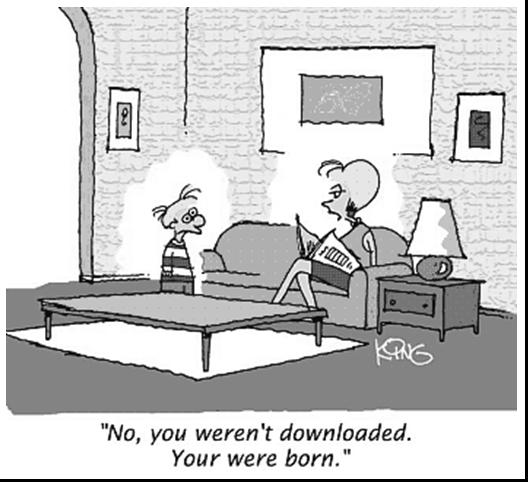
\includegraphics[width=.5\textwidth]{fig1.jpg}
\caption{A typical figure}
\label{fig:exampleFig1}
\end{figure}

\begin{figure}[ht]
\centering
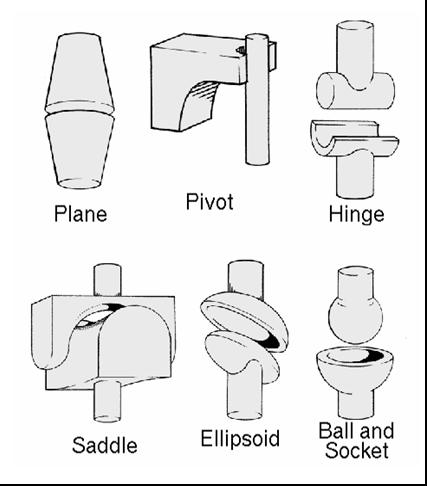
\includegraphics[width=.3\textwidth]{fig2.jpg}
\caption{This figure is an example of a figure caption taking more than one
  line and justified considering margins mentioned in Section~\ref{sec:figs}.}
\label{fig:exampleFig2}
\end{figure}

In tables, try to avoid the use of colored or shaded backgrounds, and avoid
thick, doubled, or unnecessary framing lines. When reporting empirical data,
do not use more decimal digits than warranted by their precision and
reproducibility. Table caption must be placed before the table (see Table 1)
and the font used must also be Helvetica, 10 point, boldface, with 6 points of
space before and after each caption.

\begin{table}[ht]
\centering
\caption{Variables to be considered on the evaluation of interaction
  techniques}
\label{tab:exTable1}
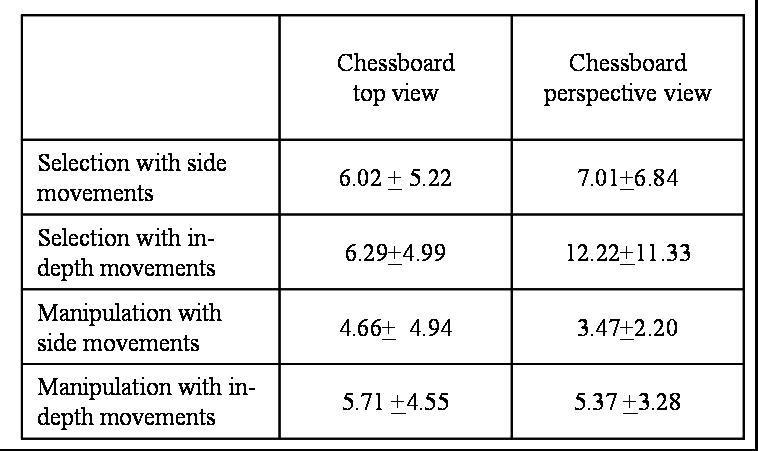
\includegraphics[width=.7\textwidth]{table.jpg}
\end{table}

\section{Avaliação de Desempenho e Benchmarks} \label{sec:desempenho}

Para validar a eficiência assintótica das estruturas e algoritmos implementados no núcleo (\texttt{core/analysis/}) e justificar o dimensionamento do grafo global, foi desenvolvido um protocolo reprodutível de \emph{benchmark} (\texttt{benchmarks/bench\_grafo.py}). Em conformidade com as restrições do projeto, a biblioteca \emph{NetworkX} é importada exclusivamente nesse módulo externo para comparação de tempo de execução e verificação automatizada de equivalência dos resultados.

Os experimentos foram conduzidos sobre grafos esparsos gerados de forma determinística (semente fixa) nos quatro tamanhos de referência definidos na modelagem: $V \in \{1.000, 5.000, 10.000, 50.000\}$ vértices, mantendo grau médio constante $\bar{d} = 8$ (correspondente a $E \in \{4.000, 20.000, 40.000, 200.000\}$ arestas não direcionadas), com topologia que combina conexões locais (formação de triângulos) e atalhos de longo alcance. Em todas as baterias, os valores produzidos pela implementação própria coincidiram integralmente com as saídas de referência do \emph{NetworkX} (diferença numérica inferior a $10^{-7}$ nas métricas contínuas e igualdade exata nos conjuntos de pontes e pontos de articulação).

\begin{table}[!ht]
\centering
\caption{Comparação de tempo de execução (em ms) entre a implementação própria e o NetworkX para grau médio $\bar{d} = 8$, e custo do passo diário de simulação.}
\label{tab:benchmark_networkx}
\footnotesize
\renewcommand{\arraystretch}{0.92}
\begin{tabular}{rrlrrr}
\hline
\textbf{$V$} & \textbf{$E$} & \textbf{Algoritmo / Operação} & \textbf{Próprio (ms)} & \textbf{NetworkX (ms)} & \textbf{Razão} \\
\hline
1.000  & 4.000   & Grau médio $O(V+E)$               & 2,10     & 0,23     & 9,31$\times$ \\
1.000  & 4.000   & Agrupamento médio $O(\sum k_v^2)$ & 5,37     & 16,88    & 0,32$\times$ \\
1.000  & 4.000   & Tarjan (pontes e artic.) $O(V+E)$ & 4,73     & 22,88    & 0,21$\times$ \\
1.000  & 4.000   & Propagação de rótulos (LPA)       & 90,55    & 45,12    & 2,01$\times$ \\
1.000  & 4.000   & Intermediação aprox.\ ($k=25$)    & 39,13    & 64,43    & 0,61$\times$ \\
1.000  & 4.000   & Intermediação exata $O(V(V+E))$   & 1.448,64 & 2.572,53 & 0,56$\times$ \\
1.000  & 4.000   & Passo diário SEIRD $O(V+E)$       & 0,23     & ---      & ---          \\
\hline
5.000  & 20.000  & Grau médio $O(V+E)$               & 13,14    & 1,21     & 10,83$\times$ \\
5.000  & 20.000  & Agrupamento médio $O(\sum k_v^2)$ & 33,56    & 85,49    & 0,39$\times$ \\
5.000  & 20.000  & Tarjan (pontes e artic.) $O(V+E)$ & 26,96    & 112,42   & 0,24$\times$ \\
5.000  & 20.000  & Propagação de rótulos (LPA)       & 524,64   & 236,21   & 2,22$\times$ \\
5.000  & 20.000  & Intermediação aprox.\ ($k=25$)    & 292,53   & 428,97   & 0,68$\times$ \\
5.000  & 20.000  & Passo diário SEIRD $O(V+E)$       & 1,10     & ---      & ---          \\
\hline
10.000 & 40.000  & Grau médio $O(V+E)$               & 29,42    & 2,42     & 12,16$\times$ \\
10.000 & 40.000  & Agrupamento médio $O(\sum k_v^2)$ & 63,87    & 166,26   & 0,38$\times$ \\
10.000 & 40.000  & Tarjan (pontes e artic.) $O(V+E)$ & 55,32    & 254,52   & 0,22$\times$ \\
10.000 & 40.000  & Propagação de rótulos (LPA)       & 1.190,54 & 647,00   & 1,84$\times$ \\
10.000 & 40.000  & Intermediação aprox.\ ($k=25$)    & 667,00   & 992,95   & 0,67$\times$ \\
10.000 & 40.000  & Passo diário SEIRD $O(V+E)$       & 2,25     & ---      & ---          \\
\hline
50.000 & 200.000 & Grau médio $O(V+E)$               & 235,38   & 12,01    & 19,59$\times$ \\
50.000 & 200.000 & Agrupamento médio $O(\sum k_v^2)$ & 404,47   & 952,45   & 0,42$\times$ \\
50.000 & 200.000 & Tarjan (pontes e artic.) $O(V+E)$ & 372,11   & 1.542,74 & 0,24$\times$ \\
50.000 & 200.000 & Propagação de rótulos (LPA)       & 6.639,63 & 3.487,40 & 1,90$\times$ \\
50.000 & 200.000 & Intermediação aprox.\ ($k=25$)    & 5.220,21 & 8.245,74 & 0,63$\times$ \\
50.000 & 200.000 & Passo diário SEIRD $O(V+E)$       & 12,33    & ---      & ---          \\
\hline
\end{tabular}
\end{table}

A Tabela~\ref{tab:benchmark_networkx} sintetiza os resultados obtidos. Observa-se que, nos algoritmos mais custosos de travessia estrutural e interseção de vizinhança --- coeficiente de agrupamento médio $O(\sum_{v} k_v^2)$, detecção conjunta de pontes e pontos de articulação de Tarjan~\cite{tarjan1972} em $O(V+E)$ e centralidade de intermediação de Brandes ---, a implementação própria superou o \emph{NetworkX}, executando entre $1{,}47\times$ e $4{,}84\times$ mais rápido (razões de $0{,}21\times$ a $0{,}68\times$). Esse ganho decorre diretamente da representação enxuta adotada no domínio: enquanto o \emph{NetworkX} armazena a topologia em dicionários aninhados de três níveis (\texttt{dict-of-dicts-of-dicts}) para acomodar rótulos genéricos e dicionários de atributos por aresta, o núcleo implementado opera sobre listas e conjuntos de inteiros contíguos ($0 \dots V-1$), reduzindo o custo de \emph{hashing} e a indireção de memória. Adicionalmente, nossa formulação do algoritmo de Tarjan unifica a extração de pontes e vértices de corte em uma única busca em profundidade (DFS) iterativa com pilha explícita, evitando duas travessias separadas e eliminando o risco de estouro do limite de recursão do Python em grafos com $V \ge 5.000$. Na detecção de comunidades por propagação de rótulos~\cite{raghavan2007}, o tempo próprio é cerca de $2\times$ superior ao do \emph{NetworkX} devido à ordenação explícita dos rótulos candidatos a cada desempate estocástico, decisão necessária para garantir reprodutibilidade estrita por semente entre execuções.

Os dados também comprovam a necessidade de substituir a intermediação exata $O(V(V+E))$ pela versão aproximada por amostragem de $k$ fontes $O(k(V+E))$ na interface da aplicação: já em $V = 1.000$, o cálculo exato demanda $1.448{,}64$~ms, ao passo que a amostragem com $k = 25$ requer apenas $39{,}13$~ms ($37\times$ mais rápida) e escala linearmente até $50.000$ vértices. Por fim, a medição da travessia diária de transmissão SEIRD confirma crescimento estritamente linear $O(V+E)$, consumindo cerca de $1{,}8$~ms por dia simulado na escala padrão de $N_{\mathrm{total}} = 8.000$ vértices ($\approx 32.000$ arestas). Combinado à execução assíncrona do motor em \texttt{QThread} e à renderização em lote via \texttt{QPainter} com histerese de ocultação de vértices ($40$~px/$36$~px), o sistema manteve média de $40$~FPS na validação de máquina, superando com folga o requisito mínimo de $20$~FPS.

\section{Limitações e Trabalhos Futuros} \label{sec:limitacoes}

Embora o grafo unificado reproduza com coerência o acoplamento entre difusão local e transporte aéreo internacional~\cite{balcan2009,brockmann2013}, o modelo apresenta limitações metodológicas e de dados que devem ser consideradas na interpretação dos resultados:

\begin{itemize}
  \item \textbf{Retrato estático da malha aérea e demografia:} as rotas do OpenFlights refletem o estado da aviação comercial até junho de 2014, enquanto a população do OWID~\cite{owid_covid_2023} corresponde a um corte único ($\approx 2022$) aplicado retrospectivamente aos surtos de 2003, 2009, 2014 e 2020. Além disso, as 13 entidades soberanas do modelo que não possuem voos internacionais registrados no OpenFlights permanecem isoladas na camada aérea, sem inserção de arestas artificiais.
  \item \textbf{Escala reduzida e topologia intranacional geométrica:} a compressão da população mundial em $N_{\mathrm{total}} = 8.000$ vértices exige que a comparação com séries reais seja feita por frações populacionais. Internamente, o grafo geométrico aleatório aproxima a contiguidade espacial, mas não captura fluxos pendulares interurbanos nem a distribuição de grau de cauda pesada associada a eventos de superdisseminação~\cite{lipsitch2003,pastor2015}; em países pequenos alocados no piso ($n_{\min} = 12$), o grau médio efetivo $\min(\bar{d}, n_i - 1)$ produz subgrafos quase completos.
  \item \textbf{Simplificações clínicas e de vigilância nos dados históricos:} o isolamento desativa todas as arestas do vértice infectado, abstraindo a transmissão intradomiciliar, e os parâmetros de intervenção e vacinação constituem premissas de cenário inspiradas na literatura~\cite{donnelly2003,ferguson2005}. No fluxo real~\cite{jhu_kaggle_covid,kaggle_ebola,kaggle_h1n1,kaggle_sars}, as séries trazem apenas casos confirmados acumulados --- sem modelagem de subnotificação e com recuperados reportados apenas no SARS (sujeitos a atraso de notificação clínica) ---, razão pela qual o mapa real adota escala sequencial de incidência por 100 mil habitantes em vez de status ativo dominante.
\end{itemize}

Como trabalhos futuros, destacam-se: (i) a inclusão de geradores topológicos livres de escala (Barabási--Albert) e de mundo pequeno (Watts--Strogatz) para modelar \emph{hubs} urbanos intranacionais~\cite{pastor2015}; (ii) a integração de redes de mobilidade pendular terrestre por modelos gravitacionais~\cite{balcan2009} para conectar fronteiras secas e países sem cobertura aérea; (iii) a adoção de redes temporais e adaptativas com redução dinâmica de tráfego aéreo durante o surto~\cite{colizza2006}; e (iv) a calibração automática multiparamétrica ($\beta, \gamma, \sigma$) por busca em grade ou inferência bayesiana sobre o erro quadrático médio das curvas históricas. 

\section{Responsabilidades dos Integrantes e Conclusão} \label{sec:conclusao}

All images and illustrations should be in black-and-white, or gray tones,
excepting for the papers that will be electronically available (on CD-ROMs,
internet, etc.). The image resolution on paper should be about 600 dpi for
black-and-white images, and 150-300 dpi for grayscale images.  Do not include
images with excessive resolution, as they may take hours to print, without any
visible difference in the result. 

\section{Referências Bibliográficas}

Bibliographic references must be unambiguous and uniform.  We recommend giving
the author names references in brackets, e.g. \cite{knuth:84},
\cite{boulic:91}, and \cite{smith:99}.

The references must be listed using 12 point font size, with 6 points of space
before each reference. The first line of each reference should not be
indented, while the subsequent should be indented by 0.5 cm.

\bibliographystyle{sbc}
\bibliography{sbc-template,referencias}

\newpage
\appendix

\section{Apêndice: Wireframes e Catálogo de Telas da Ferramenta}
\label{sec:apendice_wireframes}

Este apêndice reúne o catálogo de wireframes e especificações visuais elaborados durante o planejamento da interface com o usuário (Módulo~5). A inclusão destas telas em formato de apêndice permite documentar todo o processo de design e validação das interações do usuário, mantendo o corpo principal do artigo dentro do limite regulamentar de 12 a 15 páginas estipulado pela disciplina.

\subsection{Fluxo de Configuração e Execução da Simulação}
Apresenta as telas de parametrização da doença, calibração iterativa de $\beta$, sorteio ou escolha manual do paciente zero por país/vértice e controle temporal da execução (play, pause e velocidade).

\begin{figure}[htbp]
\centering
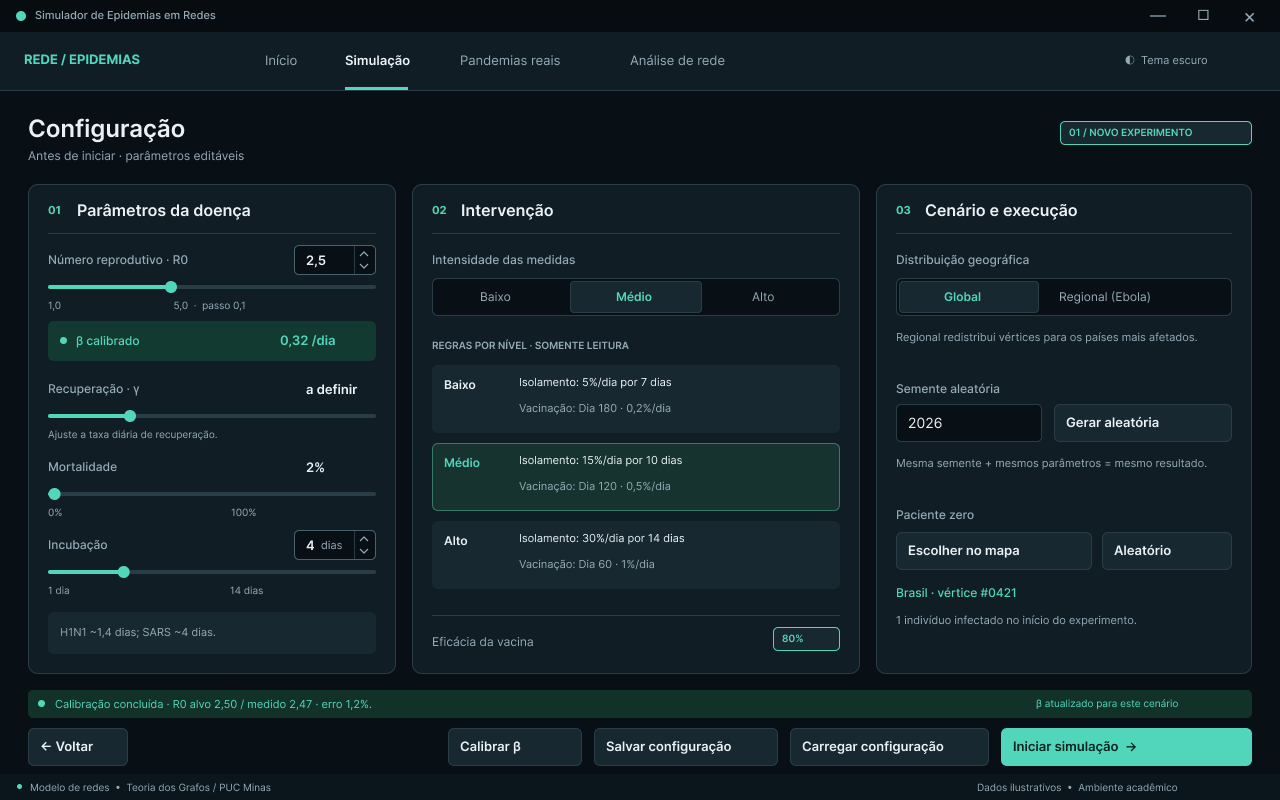
\includegraphics[width=0.85\textwidth]{figures/wf_tela02_config.png}
\caption{Wireframe da Tela 2: Painel de parametrização epidemiológica ($R_0$, $\gamma$, letalidade e níveis de intervenção).}
\label{fig:wf_tela2}
\end{figure}

\begin{figure}[htbp]
\centering
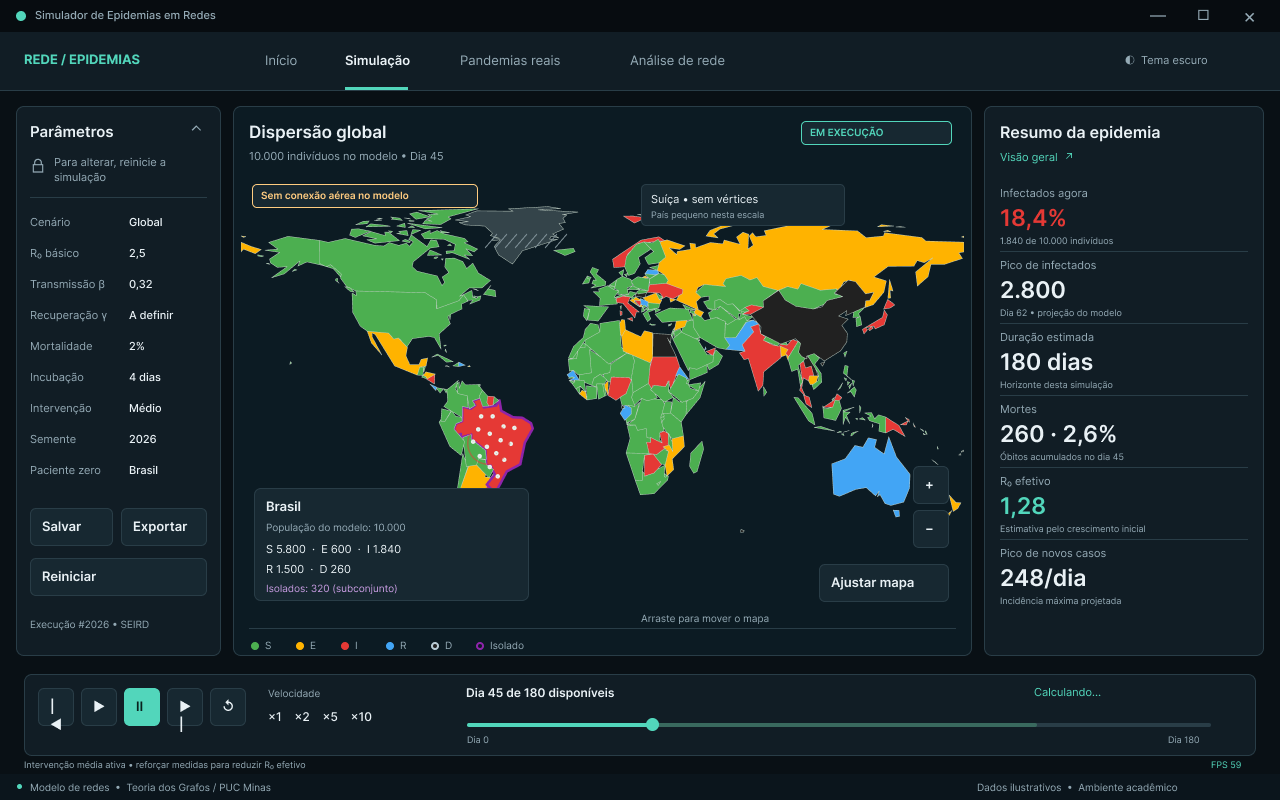
\includegraphics[width=0.85\textwidth]{figures/wf_tela05_simulacao.png}
\caption{Wireframe da Tela 5: Visualizador cartográfico global com reprodução temporal e estados SEIRD por país.}
\label{fig:wf_tela5}
\end{figure}

\subsection{Painel de Análise Estrutural de Grafos (M1 e M2)}
Reúne as telas de inspeção dos algoritmos desenvolvidos pelo grupo: componentes conexas, rotas epidemiológicas mais prováveis via Dijkstra ($-\ln p$), pontes críticas e pontos de articulação de Tarjan, métricas de centralidade e detecção de comunidades por propagação de rótulos (LPA).

\begin{figure}[htbp]
\centering
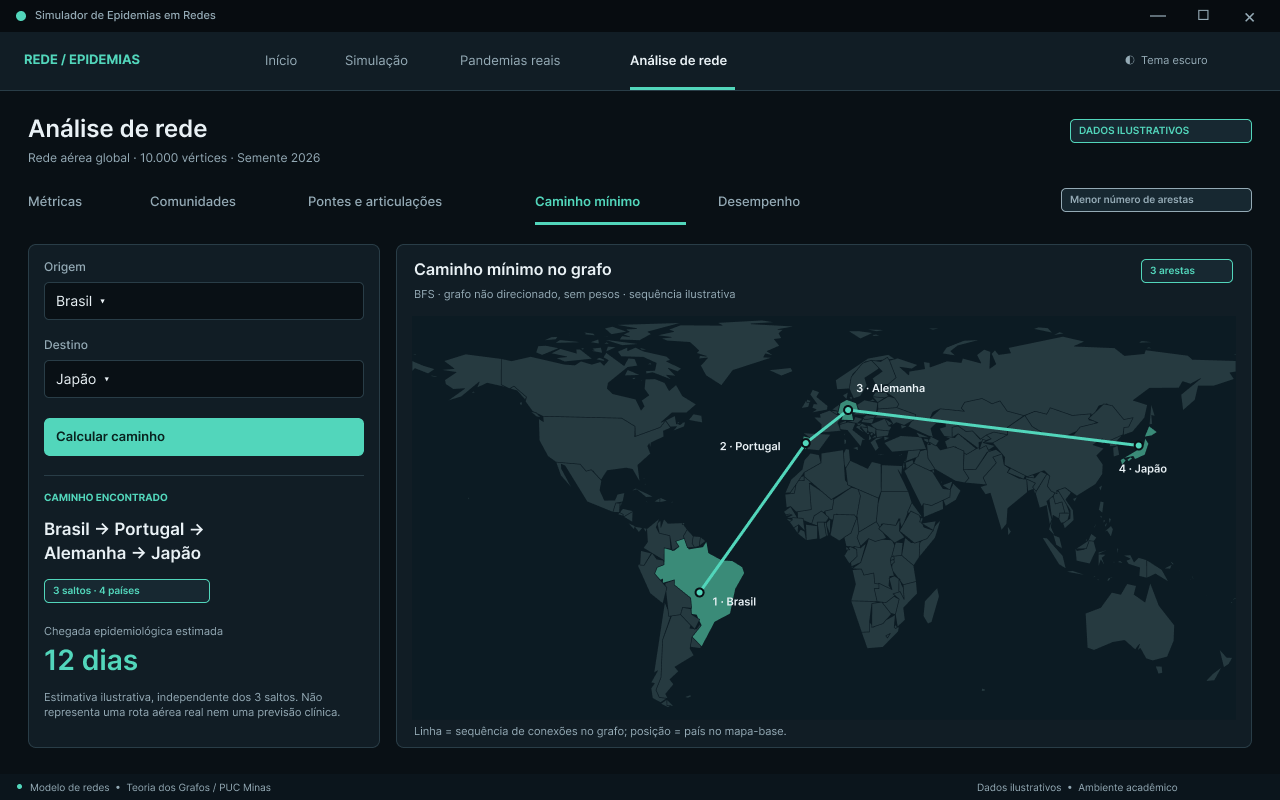
\includegraphics[width=0.85\textwidth]{figures/wf_tela10_dijkstra.png}
\caption{Wireframe da Tela 10 (Caminho Mínimo): Consulta de rotas de transmissão e probabilidade conjunta via Dijkstra.}
\label{fig:wf_tela10_dijkstra}
\end{figure}

\begin{figure}[htbp]
\centering
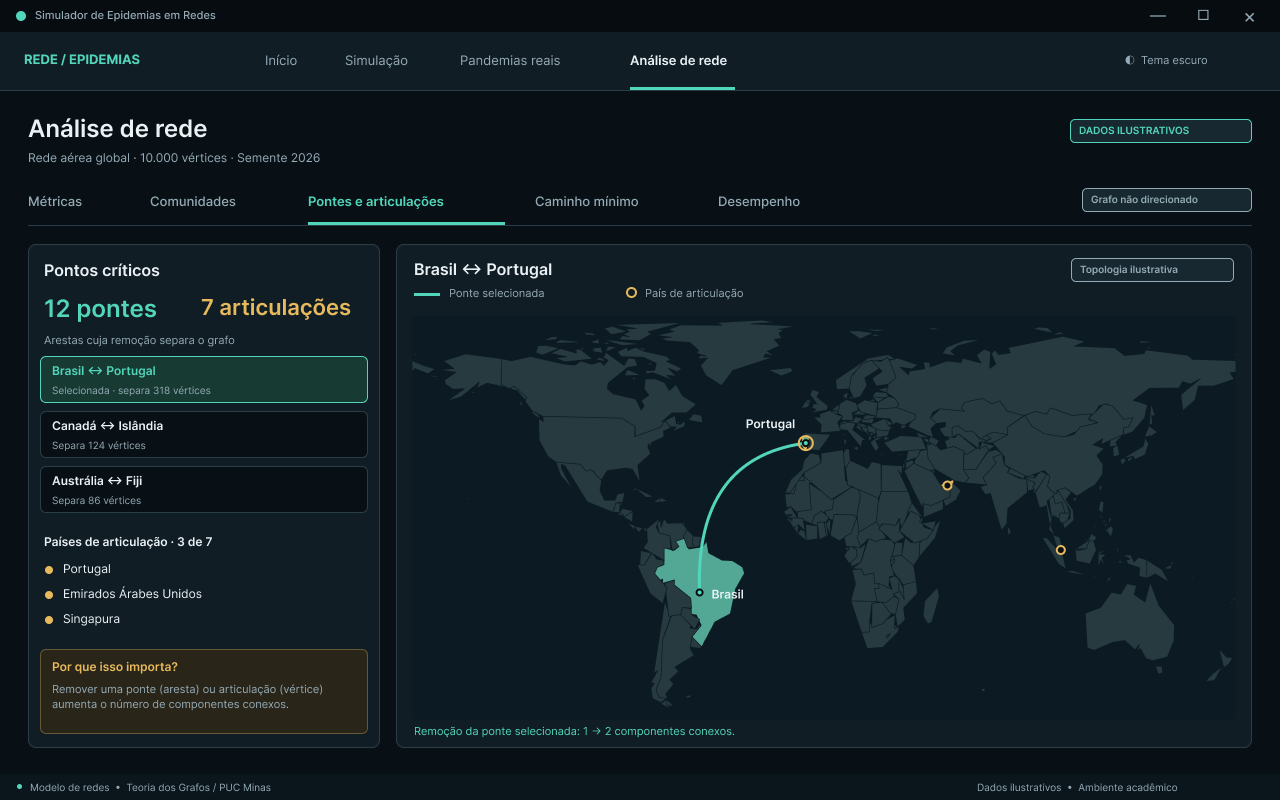
\includegraphics[width=0.85\textwidth]{figures/wf_tela10_tarjan.png}
\caption{Wireframe da Tela 10 (Vulnerabilidade): Detecção em passo único DFS de arestas de corte e vértices de articulação (Tarjan).}
\label{fig:wf_tela10_tarjan}
\end{figure}

\subsection{Fluxo de Dados Reais e Comparação Empírica (M4)}
Documenta a navegação pelos datasets históricos reais (COVID-19, SARS, Ebola e H1N1) e o painel de comparação das métricas da simulação contra curvas empíricas observadas.

\begin{figure}[htbp]
\centering
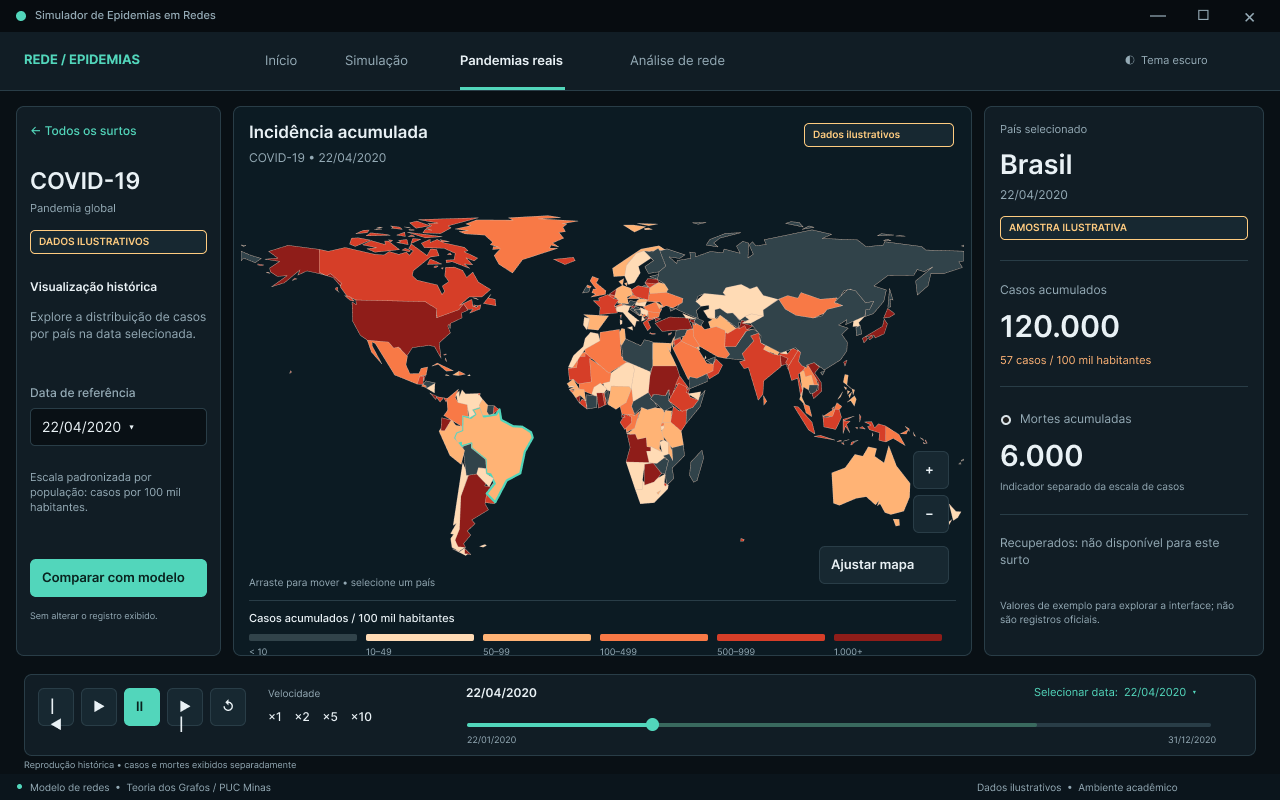
\includegraphics[width=0.85\textwidth]{figures/wf_tela09_pandemias.png}
\caption{Wireframe da Tela 9: Reprodução histórica com séries temporais oficiais e mapa coroplético de casos.}
\label{fig:wf_tela9}
\end{figure}

\begin{figure}[htbp]
\centering
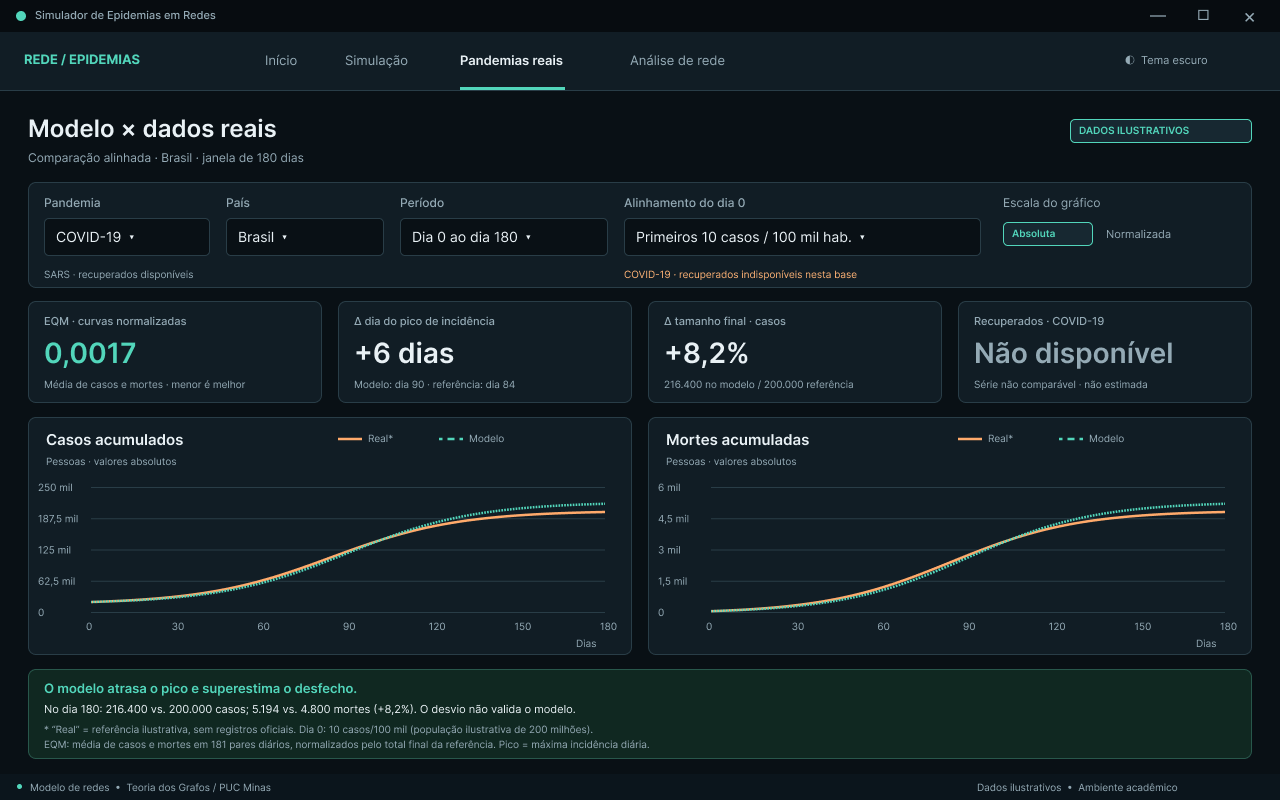
\includegraphics[width=0.85\textwidth]{figures/wf_tela11_comparacao.png}
\caption{Wireframe da Tela 11: Módulo de validação estatística e confronto entre séries sintéticas e observadas.}
\label{fig:wf_tela11}
\end{figure}

\subsection{Telas Complementares e Inspeção Detalhada}
Inclui o visualizador de inspeção de vértice individual no mapa (país, grau $k_v$, coeficiente de agrupamento local $C_v$ e vizinhos ativos), além dos diálogos de persistência de configuração e exportação de dados em CSV.

\begin{figure}[htbp]
\centering
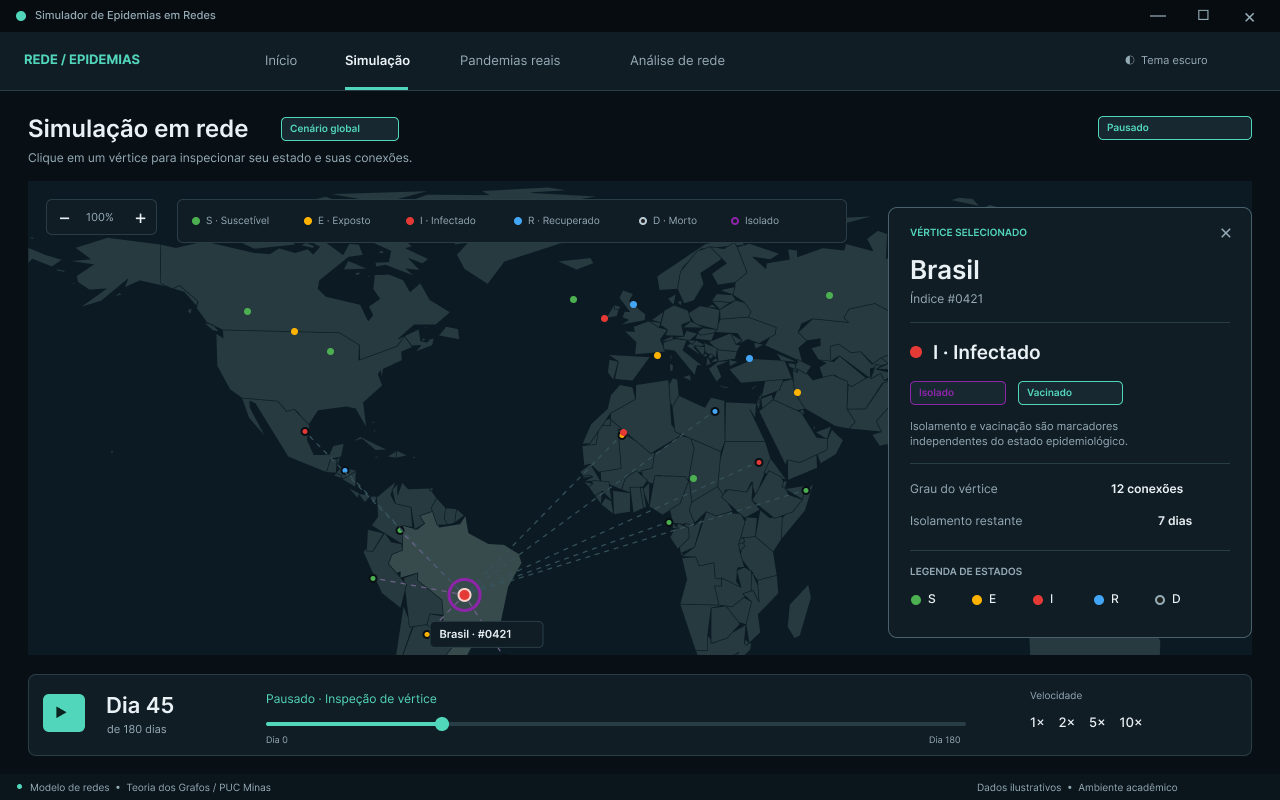
\includegraphics[width=0.85\textwidth]{figures/wf_tela14_inspecao.png}
\caption{Wireframe da Tela 14: Inspeção pontual de vértice por clique no mapa interativo.}
\label{fig:wf_tela14}
\end{figure}

\end{document}
